\documentclass[12pt]{article}

\usepackage[utf8]{inputenc}
\usepackage[T1]{fontenc}
\usepackage{geometry}
\usepackage{graphicx} %figures
\usepackage{subfig} %subfigures
\usepackage{gensymb} %degree sign
\usepackage{amsmath} %math stuff
\usepackage{bm} %bold stuff
\usepackage[]{algorithm2e} %algorithms
\geometry{a4paper}

\title{\textbf{Part 6: MCMC and Bayesian Modeling Part II}}

\begin{document}
\date{January 11, 2021}
\maketitle

If you recall the post on January 4, 2021 discussing the basics of Bayesian modeling using Gibbs and Hamiltonian-Monte Carlo Sampling (HMC), both use \emph{Bayes Rule} with a prior $\pi(\theta)$ over the parameter and a likelihood $p(x|\theta)$:

\begin{equation}
Pr(\theta | x) = \propto \pi(\theta) p(x | \theta)
\end{equation}

\vspace{5mm}

Here we will go over some fun examples of using this simple rule to solve a variety of problems!

\section{A Probit Model for Death Probability}

Let's say we have a binary classification problem $y\in [1,0]$ where we have indicator variables $X = [1,x_{age},x_{gender}]$ ($1$ is for a bias/intercept) where $y_i=1$ indicates a person died and $x_{gender}=1$ indicates a person was male (in the example I took this from it's the \emph{Donner Party} survival statistics). First we need a mathematical model. We shall use the probit model where $\Phi$ is the standard normal probability density function (which will utilize a linear model $\beta^T x_i = \beta_0+\beta_1 x_{i,1}+\beta_2 x_{i,2}$):

\begin{equation}
Pr(y_i=1|x_i)=\Phi(\beta^T x_i)
\end{equation}

\vspace{5mm}

It may be obvious to smart people, of which I am not, but the likelihood function for this model is as follows:

\begin{equation}
L(x_i,X,Y,\beta)=\Pi_i^N \Phi(\beta^T x_i)^{y_i}(1-\Phi(\beta^T x_i))^{1-y_i}
\end{equation}

\vspace{5mm}

We can use a simple non-regularizing prior:

\begin{equation}
Pr(\beta) = 1
\end{equation}

I will write out the full HMC algorithm for everyone here (also check the code attached):

\vspace{5mm}

\begin{algorithm}[H]
 \KwData{$p(\beta)$ Posterior Equations}
 \KwResult{$B \sim Pr(\beta)$ Posterior Sample}
Initialize $\theta$\;
\For{$k = 1:K$ Samples}{
$\beta_p \sim N(\beta,I)$\;
$p(\beta) = 1\times L(X,Y,\beta)$\;
$p(\beta_p) = 1\times L(X,Y,\beta_p)$\;
$q(\beta |\theta_p) = N(\beta | \mu=\beta_p, I)$\;
$q(\beta_p | \beta) = N(\beta_p | \mu=\beta, I)$\;
$\alpha = min\{1,\dfrac{p(\beta_p) q(\beta | \beta_p)}{p(\beta) q(\beta_p | \beta)}\}$\;
$Pr(\beta = \beta_p = B_k) = \alpha$\;}
 \caption{Hamiltonian-Monte Carlo Sample}
\end{algorithm}

\vspace{5mm}

\begin{figure}[h]
\centering
\subfloat[Chains]{\raisebox{2ex}
{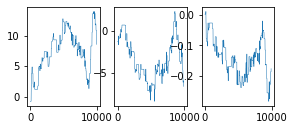
\includegraphics[width=0.3\textwidth]{Post_6_ex1}}}
\subfloat[][Posterior of $\beta$]{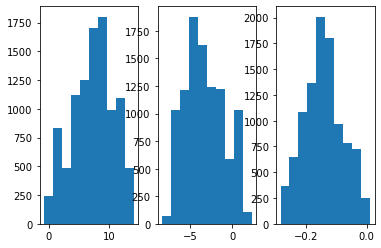
\includegraphics[width=0.3\textwidth]{Post_6_ex2}}
\subfloat[][Posterior of $Pr(y=0|x)$ for Males]{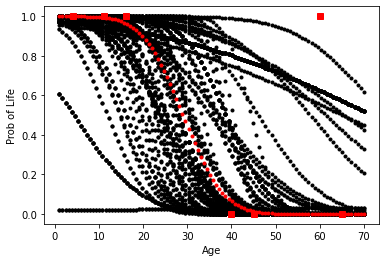
\includegraphics[width=0.3\textwidth]{Post_6_ex3}}
\caption{Bayesian Probit Model for Survival}
\end{figure}

\vspace{5mm}

Where the parameters for the probit model are $\beta=[\beta_0,\beta_{age},\beta_{gender}]$. We find from Figure 1(b) that the distribution of the model parameters are $\beta_{age},\beta_{gender}<0$. This indicates that being older and a male are correlated with the outcome $Pr(y_i=1|x_i)$ (death). The theory is that older people are weaker and women have more body-fat / weight than men, so younger people and women were more likely to survive the \emph{Donner Party}. 

\section{Gaussian Process Model Solved using HMC}

Now let's look at the Gaussian process model (GP) from our first official post! Remember the mean $\hat{\mu}$ and standard deviation $\hat{\sigma}^{2}$ of the model is in the following form:

\begin{equation}
\hat{\mu} = K(x,X)(K(X,X) + \sigma^{2}I)^{-1}Y
\end{equation}
\begin{equation}
\hat{\sigma}^{2} = K(x,x) - K(x,X)(K(X,X)^{-1}K(X,x)
\end{equation}

\vspace{5mm}

Where we have a kernel matrix $K(x,x')$ that relates a point $x$ to another point $x'$ (usually through a Euclidean distance metric). If you also recall, the likelihood function is as follows:

\begin{equation}
L(\sigma,\sigma_{f},l) = -0.5YK_{y}Y^{T} - 0.5log(det(K_{y}))-0.5nlog(2\pi)
\end{equation}
\begin{equation}
K_{y} = K(X,X)+\sigma^2 I
\end{equation}

\vspace{5mm}

Well, we have a likelihood, all we need is a prior. Let's use the same non-regularizing priors as in Equation (4). Let's train our model on input data $X$ and output data $Y$ using $N=8$ data points for the test function $f(x_1,x_2)=x_1-x_2+U(0,0.1)$. To be clear, we are "training" using the HMC algorithm detailed in the previous post with the posterior:

\begin{align*}
Pr(\sigma,\sigma_{f},l|X,Y)=L(X,Y|\sigma,\sigma_{f},l)Pr(\sigma)Pr(\sigma_f)Pr(l)
\end{align*}

\vspace{5mm}

This one was a little harder to solve with an extremely generic HMC algorithm (no fancy tricks that \emph{stan} might use) but using $M=10^5$ HMC iterations and a proposal distribution of $Pr(\beta_p|\beta)=N(0,10^{-3}I)$ for all parameters $\beta$ I was able to get reasonable regression (by shrinking the proposal distribution variance, the Markov Chains are less likely to move in extreme directions). The results in Figure 2 show at least reasonable estimates, which points in the direction that we are on the road to building our own HMC algorithms!

\vspace{5mm}

\begin{figure}[h]
\centering
\subfloat[][Data]{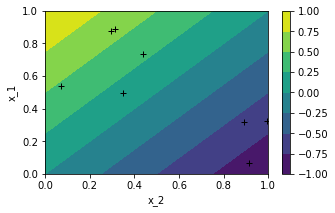
\includegraphics[width=0.3\textwidth]{Post_6_gauss1}}
\subfloat[][GP with HMC Solved $\theta$]{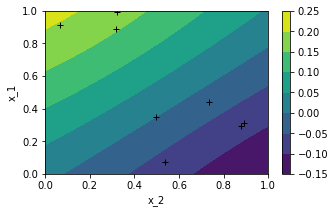
\includegraphics[width=0.3\textwidth]{Post_6_gauss2}}
\caption{GP Test Problem Results}
\end{figure}

\vspace{5mm}

The results for the chains are not perfect. In fact while the distributions may show a clustering around particular means, and the final results for regression aren't terrible, the dynamics of the chains are a different story.

\begin{figure}[h]
\centering
\subfloat[Chains]{\raisebox{2ex}{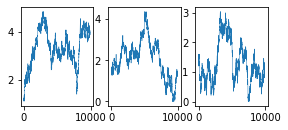
\includegraphics[width=0.3\textwidth]{Post_6_gauss3}}}
\subfloat[][Posterior of $\theta$]{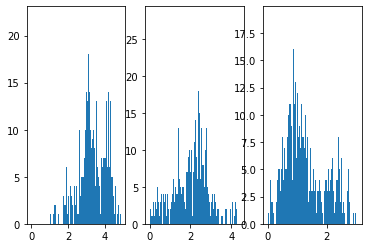
\includegraphics[width=0.3\textwidth]{Post_6_gauss4}}
\caption{HMC Posterior Results}
\end{figure}

\section{Convergence and Output Analysis}

The primary means of analysis of convergence (or the stationarity) of the posterior is via the Gelman-Rubin approach. In this approach we calculate the metric:

\begin{equation}
\hat{R}= (\dfrac{V(B|X)}{W})^{1/2}
\end{equation}

\begin{align*}
V(B|X)=\dfrac{K-1}{K}W+\dfrac{1}{K}b
\end{align*}

\begin{align*}
b = \dfrac{K}{M-1}\Sigma_j^M (\hat{B}_{.j}-\hat{B}_{..})^2
\end{align*}

\begin{align*}
W = \dfrac{1}{M}\Sigma_j^m s_j^2
\end{align*}

\begin{align*}
s_j^2 = \dfrac{1}{K-1}\Sigma_i^K (B_{ij}-\hat{B}_{.j})^2
\end{align*}

\begin{align*}
\hat{B}_{.j} = \dfrac{1}{K} \Sigma_i^K B_{ij}
\end{align*}

\begin{align*}
\hat{B}_{..}=\dfrac{1}{M} \Sigma_j^M \hat{B}_{.j}
\end{align*}

\vspace{5mm}

Yes I know that's a lot (and it is). So go through the code where I make each of these calculations step by step and see what's going on here. The variable $b$ and $W$ are two measures of variance. For our analysis we break each chain into two chains for a total of $M$ chains. We don't utilize 'burn-in' period in which we ignore the first (usually $0.25K$) few posterior solutions. In our example problem let's use HMC on the GP problem above with $K=100$ samples, five chains for a total $M=10$. 

\begin{figure}[h]
\centering
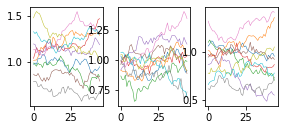
\includegraphics[width=0.7\textwidth]{Post_6_gauss5}
\caption{HMC Chains for GP Problem}
\end{figure}

\vspace{5mm}

Notice that the chains are kind of everywhere, but that is all relative. We are really just trying to get a feel for the math and simulation behind MCMC and not spend time doing perfect implementation. I'll just say here (i) we'd want to have a burn-in period, (ii) we'd want a stronger algorithm (such as the powerful NUTS Sampler used in PYMC3) and/or (iii) better use of priors. 

\vspace{5mm}

Finally we have the solution to the GP problem in $\hat{R}$ (In general you want $1.1<\hat{R}<1$):

\begin{align*}
\hat{R} =
\begin{pmatrix}
1.4 \\ 1.3 \\ 1.5
\end{pmatrix}
\end{align*}

\vspace{5mm}

Done for today. We will be leaving MCMC for now and next week we'll go over a fun global optimization method: Trust Regions!

\end{document}